در این روش همسایه‌های state فعلی بررسی می‌شوند.
اگر همسایه‌ای وجود داشته باشد که h آن کمتر از state فعلی باشد، آن state را به عنوان state بعدی انتخاب خواهیم کرد.
الگوریتم زمانی پایان می‌یابد که چنین همسایه‌ای یافت نشود و یا در مسائل goad-satisfaction به هدف مدنظر برسیم.

در واقع این روش را می‌توان به صعود کردن به قله اورست توسط یک فرد نابینا و در هوای مه‌آلود تشبیه کرد.
منظور از نابینایی این هست که ما برای انتخاب state های بعدی انتخاب‌های کمی داریم و تنها می‌توانیم در هر قدم همسایگان حالت فعلی را بررسی کنیم و منظور از هوای مه‌آلود آن است که الگوریتم حافظه‌ ندارد و ممکنه است به یک state چندین مرحله برگردد.

\begin{figure}[H]
    \centering
    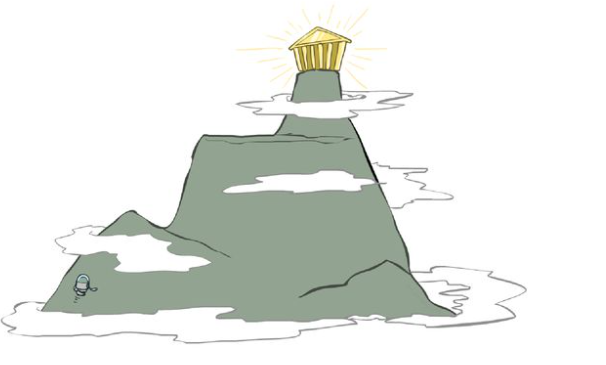
\includegraphics[width=0.5\textwidth]{source/everest-climbing}
    \label{fig:hill-climbing}
\end{figure}

\subsubsubject{بررسی مسئله 8 وزیر به کمک روش hill-climbing}{files/8-queen-hill-climbing.tex}
